\documentclass[conference]{IEEEtran}
%\IEEEoverridecommandlockouts
\usepackage{epstopdf}
\usepackage{caption}
\usepackage{float}
\usepackage{booktabs}
%\usepackage{subcaption}
\usepackage{amsmath}
\usepackage{amsfonts}
\usepackage{amssymb}
\usepackage{amsbsy}
\usepackage{subfig}
\usepackage{algorithm}
\usepackage{varwidth}% http://ctan.org/pkg/varwidth
\usepackage{gensymb}
\usepackage[noend]{algpseudocode}
\usepackage[export]{adjustbox}
\usepackage{todonotes}
\usepackage{verbatim}
\usepackage{multirow}
\graphicspath{{./images/}}


\usepackage{acronym}
\acrodef{TTE}{Travel Time Estimation}
\acrodef{RSP}{Road Speed Profiles}
\acrodef{ATMS}{Advanced Traffic Information and Management Systems}
\acrodef{OSM}{Open Street Map}
\acrodef{CH}{Contraction Hierarchies}
\acrodef{FCD}{Floating car data}
\acrodef{ML}{Machine Learning}
\acrodef{OD}{origin-destination}
\acrodef{EMA}{Exponential Moving Average}
\acrodef{CoV}{Coefficient of Variation}
\acrodef{EDT}{estimated driven distance}
\acrodef{MAPE}{Mean absolute percentage error}
\acrodef{RMSE}{Root mean square error}
\acrodef{POI}{Point of Interest}
\begin{document}



\title{Road Speed Profiling for Upfront Travel Time Estimation
}
%\begin{comment}
\author{\IEEEauthorblockN{Abhinav Sunderrajan, Jagannadan Varadarajan, Kong Wei Lye}
\IEEEauthorblockA{\textit{Data Science, GrabTaxi Holdings Pte. Ltd, SINGAPORE}\\
\{abhinav.sunderrajan,jagan.varadarajan,kongwei.lye\}@grab.com}

}
%\end{comment}

% The paper headers
\markboth{Road speed profiling for upfront travel time estimation}%
{Shell \MakeLowercase{\textit{et al.}}: Bare Demo of IEEEtran.cls for IEEE Journals}

% make the title area
\maketitle

\begin{abstract}
 Accurate travel time estimation is crucial for several service based industries such as ride hailing, food delivery, logistics etc. Promises made to the passengers in terms of cab allocation, waiting times and food delivery times need to be kept to avoid passenger churn given the number of competing start-ups in these sectors. Further, travel times impact the cost of the cab rides and delivery charges which are shown upfront to the passengers and drivers. Trip time estimations must thus be very accurate to avoid both passenger and driver disenchantment. In this paper we present a solution for accurate upfront \ac{TTE} based on \ac{RSP} and a corrective \ac{ML} model using data from around $\bf{9.5}$ million taxi trips in two (each) mega-cities in S.E Asia. 

\end{abstract}


% Note that keywords are not normally used for peer-review papers.
\begin{IEEEkeywords}
Road speed profiling, travel time estimation, machine learning
\end{IEEEkeywords}


\IEEEpeerreviewmaketitle

\section{Introduction}
\label{sec:intro}
The problem of \ac{TTE} has been receiving enormous interest over the past few years as it forms the fundamental building block in  applications such as route planning, traffic dispatching, cost estimation and ride dispatching used in navigation engines, ride-hailing, food delivery and logistics. Although \ac{TTE} is a well studied problem over several years, the increased availability of several traffic related data-streams from various sources such as smart phones, vehicles and sensors along with big-data infrastructure (e.g. Apache Kafka) opens the possibilities for collection, management and analysis of vast amounts of GPS probe data. Measuring point-to-point travel time estimates and building \ac{ATMS} could eventually help ease congestion given the constraints in terms of building new infrastructure.



There are several challenges towards accurate \ac{TTE}. Primary among those are noisy GPS data which makes it hard to estimate the exact location of vehicles especially in {\it urban canyons} with tall skyscrapers preventing effective GPS signal reception. Furthermore, in several cities, the map data like those from \ac{OSM} is rather inaccurate with several missing roads. Another challenge with using \ac{FCD} for \ac{TTE} is the sparsity of probe vehicle penetration. Several studies estimate a minimum of $2\%$ to $5\%$ for accurately determining traffic state and thereby inferring travel times.

Another crucial aspect in aggregating the speed of vehicles on roads is that vehicle speeds are inherently stochastic. We can notice vehicles in different lanes travel at different speeds (discounting various driver behaviours) depending upon the intended route. The randomness in road speeds is especially significant during peak hours as discussed in Section~\ref{subsec:speed-disribution}. Accurate lane level map matching is very challenging thus making it even harder to infer travel times. Finally, we also need to take into account dynamic changes to traffic conditions due to events such as accidents, road closures and thunder storms making accurate \ac{TTE}, a hard problem to solve. 

Approaches for TTE are broadly categorized as \emph{individual} and \emph{collective} based on the input data used in estimating TTE. In the individual approach, a given route is first split into several road  segments for which a travel time estimate is accurately calculated using (either pre-calculated or real-time or both) speed profiles of individual road segments. The final TTE is given simply as the sum of the travel times of the constituent segments. Earlier works such as~\cite{de2008traffic} and~\cite{nanthawichit2003application} fall in this category.
%

While collective methods can estimate individual travel times (via speed profiles) accurately, they ignore complexities arising due to road intersections, traffic lights, and turns. Hence, they additionally need  explicit models to capture time spent in the aforementioned overheads. However, individual methods appear to be more elegant while building large scale systems that should incorporate both historical and real time data.  
%
On the other hand, collective approaches  directly estimate the travel time for the entire path by implicitly considering inputs including the path length, time and day. Collective approaches are typically easier to build as they can be agnostic to the underlying routing constraints. However, their accuracy will vastly depend on the quality and coverage of historical data. The work in~\cite{jenelius2013travel} is an example of a collective method where the authors use \ac{FCD} to develop network models for estimating intersection delay and estimate spatio-temporal correlation between neighbouring links.


In this paper, we present a hybrid approach to \ac{TTE} that combines the advantages of both \emph{individual} and \emph{collective} methods. Our method operates on two phases: in the first phase, we compute an \emph{initial TTE} for a given origin-destination (OD) pair by relying on (historical) road speed profiles of the constituent road segments. However, since this initial TTE does not account for time delays encountered in traffic lights, intersections and turns,  in the second phase, we use a collective approach, where a \emph{final TTE} is predicted using a corrective machine learning (ML) model that takes the initial \ac{TTE}, along with time and day features as input. 

The first step in deriving an initial TTE is modeling \ac{RSP} for every road segment in the city's road network using our GPS probe data -- we use \ac{OSM} definition of road segments for our modeling purpose here. Road speed profile can be roughly defined as the expected speed of a vehicle for a particular road segment at given time and day. While we use \ac{RSP} only as intermediate result here, they are also widely used to detect abnormalities such as speeding cars, and traffic events~\cite{asakura2015incident}. 

By their very nature, \ac{RSP} exhibit huge variations owing to changes in vehicle speeds on the same segment over time, and the variety of GPS probe devices used to collect our observations (most of the ride-hailing cabs in Southeast Asia use cheap mobile phones with poor GPS receivers) An important problem here is to define the time intervals on which RSPs should be defined. Whereas most common way to capture historical speed profiles is by accumulating observations over pre-defined time buckets, they may not yield the best results, a simple \emph{one size fits all}  bucket may not be suitable for every time of the day. For instance, speed profiles during peak hours tend to have larger variations requiring finer time buckets, while non-peak hours tend to have very few rides, hence needing longer duration for reliable \ac{RSP}. To address this issue, we propose a regression tree based dynamic time buckets that adjust the time intervals based on the number of rides instead of just time.    

More precisely, the contributions of this paper are multi-fold: 
\begin{enumerate}
	\item We present a simple, yet effective approach to derive \ac{RSP} using \ac{FCD} from ride hailing cabs. 
	\item In order to capture speed profiles from historical data both in terms of their variance and coverage during different time intervals of the day and week, we propose an to use a decision tree based adaptive time buckets (detailed in section~\ref{subsec:adaptive-buckets}).
	\item We propose to employ a corrective \ac{ML} algorithm to implicitly model delays due to traffic lights, intersections, turn and other traffic events. The initial TTE from speed profiles will form an input to the corrective ML model. 
	\item Finally, we illustrate the effectiveness of our approach using a millions of rides done over a month in two mega-cities of Southeast Asia. To the best of our, this is one of the first attempts to study traffic patterns and travel times in S.E Asia using such as large scale data set.    
\end{enumerate}

The reminder of this paper is organized as follows: After providing the definitions for \ac{RSP} in the following section, we detail our approach to model \ac{RSP} in Section~\ref{sec:road-speed-profiling-details}.
%we discuss in detail the work-flow for constructing the \ac{RSP}. Specifically we talk about identifying pickup and drop off locations of a cab ride, . distribution of vehicle speeds and finally providing an \ac{EMA} based \ac{RSP} for each road segment on the road network graph. %
In Section~\ref{sec:travel-time-estimation} we discuss how we use the initial output of \ac{RSP} to give a final \ac{TTE} using a corrective ML model. 
In Section~\ref{sec:experiments}, we provide extensive experimental results of our approach on trips made in two mega cities of S.E Asia, hereafter referred to as City~$1$ and City~$2$ \footnote{We are avoiding specifying names of the cities deliberately.} for both pickup and drop off phases of a cab ride. The paper concludes in Section~\ref{sec:conclusion}. 



\section{Road speed profiles}
\label{subsec:road-speed-profile}

Road speed profiling refers to the process of computing the expected, median, upper-bound and lower-bound (within a confidence interval) speeds of road segments in a city at a given time of the day. 
More precisely: $\mathbf{G(V,E)}$ represents the road network of a city modelled as a directed graph. Here, $V$ and $E$ represent the set of vertices (nodes) and edges respectively. Here, edges represent road segments and nodes represent intersections. Note that we will used the terms edge and road segments interchangeably. The edge weights represent a metric of interest, which is often either the length of the road segment or the time take it takes to travel through it, i.e. speed profile. 

Given the set of road segments $E = \{e_i\}_{i=1}^{N}$, and time buckets indexed by $t =\{1,2,\ldots, T\}$, \ac{RSP} involves estimating the expected speed profile $\mu_{e_i,t}$, and its median $\bar{\mu}_{e_i,t}$, upper bound $\mu^{upper}_{e_i,t}$ and lower bound $\mu^{lower}_{e_i,t}$ for each edge $e_i$ and time interval $t$. The confidence intervals representing the upper and lower bound speeds represent the $68\%$ confidence intervals using the \emph{Gosset's t-distribution} with $n-1$ degrees of freedom. Here $n$ is the number of vehicles speed samples for edge $e_i$ in time interval $t$.


Computation of \ac{RSP} initially involves reliably {\it map matching}~\cite{quddus2007current,sunderrajan2014map} driver trajectories on to a digital road network to extract the distribution of the speeds of the vehicles traversing a given road. We are using \ac{OSM} to construct our road network graphs for City~$1$ and City~$2$ each containing close to $71k$ and $118$k edges respectively. Given the large number of road segments we need to ensure that most of them are sufficiently traversed by taxis to ensure adequate spatio-temporal coverage.






\section{Methodology of road speed profiling}
\label{sec:road-speed-profiling-details}

\begin{figure}[!tb]
	\centering
	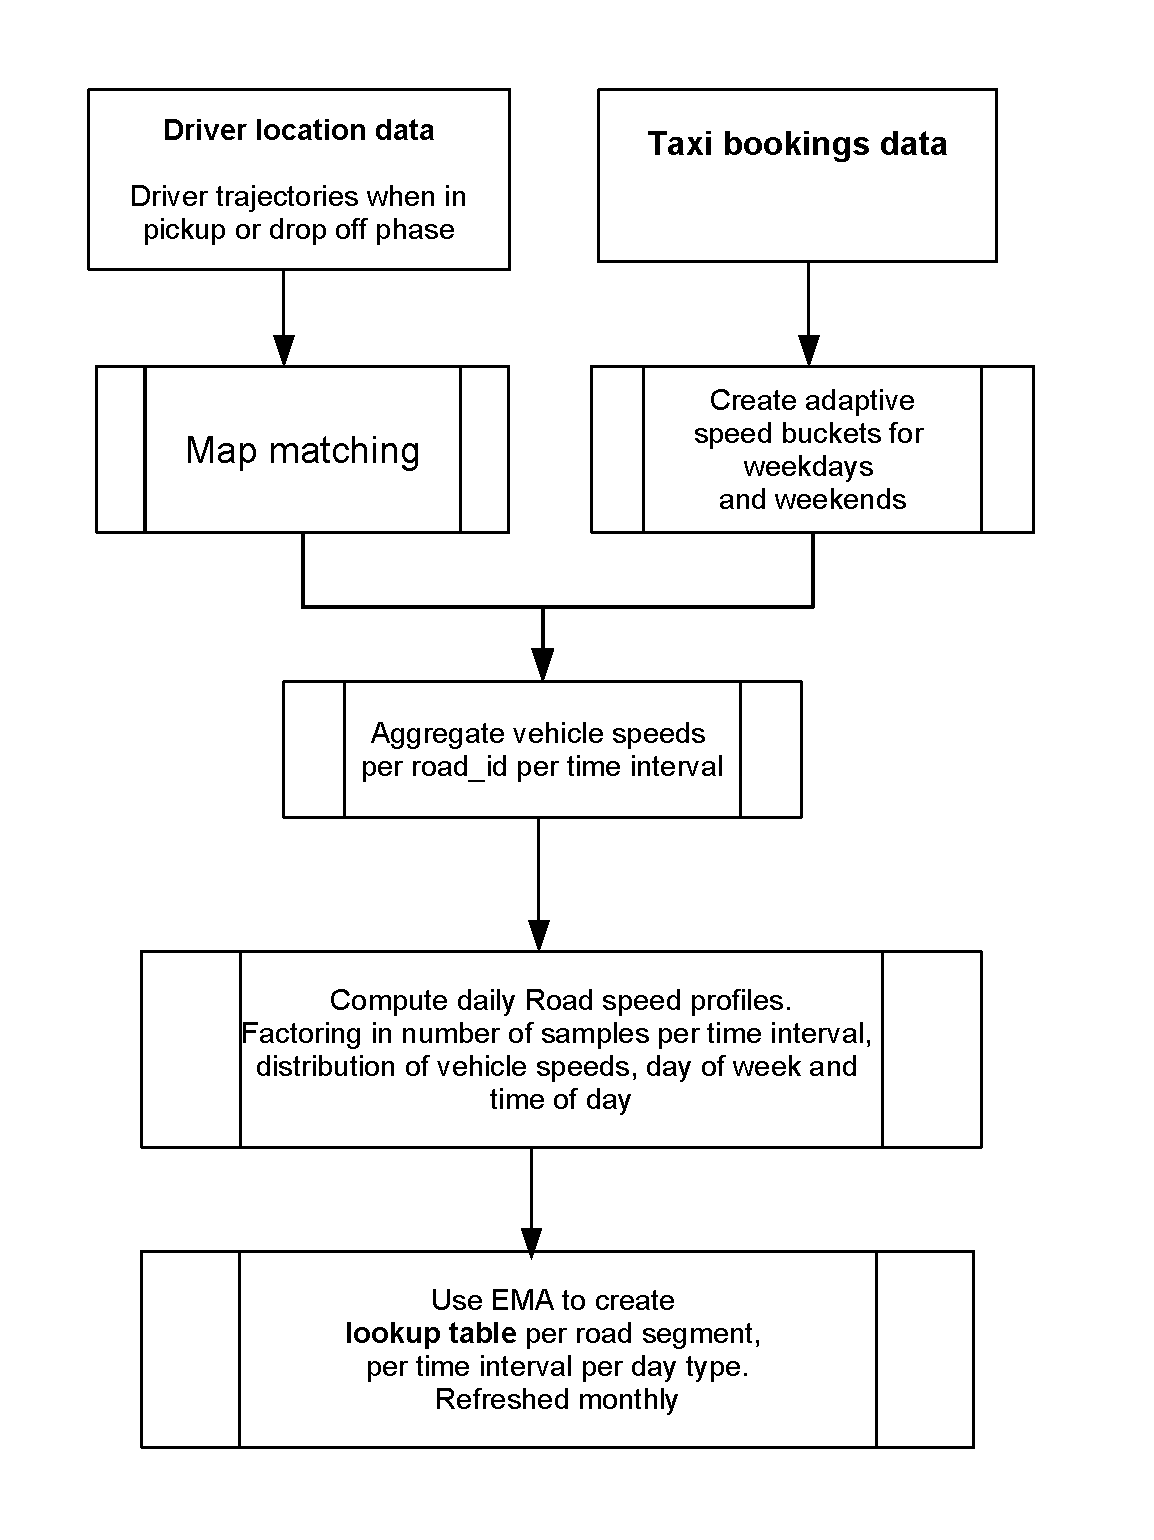
\includegraphics[width=\columnwidth,left,height=7.5cm,keepaspectratio]{images/WorkFlowRSP.pdf}
	
	\caption{Work flow for road speed profiling.}
	\label{fig:workflow-rsp}
\end{figure}



Figure~\ref{fig:workflow-rsp} presents our work-flow to compute \ac{RSP} by processing the massive driver trajectory data-set. The steps involved in RSP computation are:
\begin{enumerate}
    \item Identify if the driver is on a job (either pickup or drop off phase of a ride). We discount GPS probes when drivers are not on a job as they may not be representative. 
    \item Map-matching driver trajectories, extract the vehicle speed distribution across road segments.
    \item Identify time bucket using the time stamp and pre-calculated adaptive time buckets for weekdays and weekends.
    \item Extract the distribution of road speeds for each road per time bucket.
    \item Computation of \ac{EMA} of road speeds.
\end{enumerate}


\subsection{Map-matching driver trajectories}
\label{subsec:snap-to-road}
Map-matching or snapping driver trajectories to road segments is the process of integrating the noisy driver GPS data and the spatial road network data in order to identify the exact road segment or link in which the vehicle is traversing. Thanks to several years of research in this area, the performances of these algorithms have steadily improved due to advances in inference techniques and improvements in the quality spatial road network data. 

We use the map-matching algorithm presented in~\cite{newson2009hidden} with two main improvisations: a) we also make use of the bearing (orientation of a moving vehicle to true north) information to improve accuracy. 2) use contextual information to identify the correct link when equi-probable paths (e.g., highway and road underneath) are encountered.  

\subsection{Adaptive speed buckets}
\label{subsec:adaptive-buckets}
The time intervals into which we choose to bin the $1440$ minutes constituting a day plays an important role in inferring road speed distributions. 
%
Conventionally used time buckets, e.g., one hour or half an hour, which amounts to $24$ and $48$ time bins in a day tend to be less adaptive to the traffic flow in the city and the resulting variations. For example, a shorter time bucket such as 30 minutes can be adequate for peak-hour traffic flow, but may have sparse spatio-temporal coverage during AM and PM non-peak hours. Furthermore, it results in $48$ contracted graphs for a single day making the downstream routing algorithms such as \ac{CH}~\cite{geisberger2012exact,luxen-vetter-2011} non-scalable. 

 
%(since the edge weights of the routing graphs will be travel times across them). This is a big number for production systems handling several millions of routing calls every second. 



\begin{figure}[!tb]
	\centering
	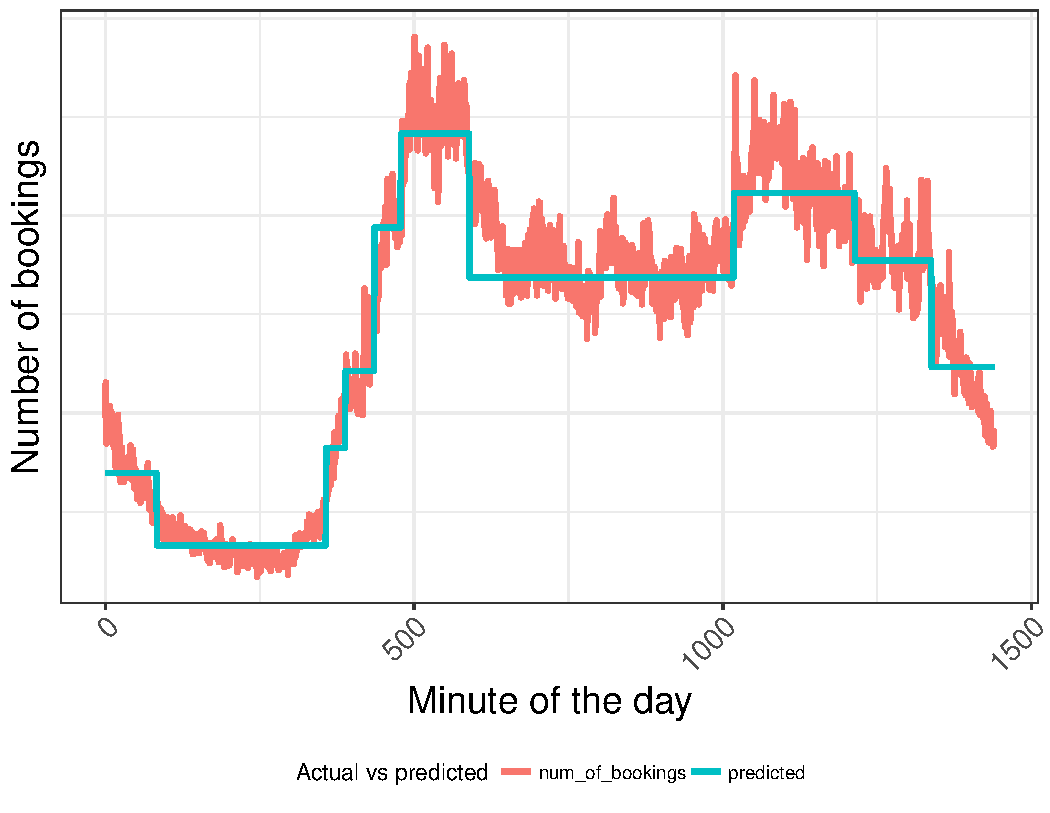
\includegraphics[width=\columnwidth,left,height=6cm,keepaspectratio]{images/AdaptiveBinning.pdf}
	
	\caption{Adaptive time bucketing: Predicting the number of bookings at any time of the day with minute of the day being the only feature.}
	\label{fig:adaptive-binning}
\end{figure}
 
Moreover, typically traffic flow in any city will have distinct peak hours, where the variance in traffic flow is high. The speeds of roads vary sharply with onset and offset of congestion. On the contrary, we  find the traffic conditions are fairly static during non-peak hours, e.g., between $01$:$00$ and $03$:$00$ hours barring exceptions such as accidents and road closures. 


In order to address problems in manually choosing the time intervals, we propose to use a data-centric approach to partition a day into \emph{adaptive time buckets} for further \ac{RSP} computation. 
To this end, we implemented a \emph{decision tree} based regression algorithm to partition the day based on travel patterns observed in the city.

 
The \emph{decision tree} (DT) uses the time (in minutes of the day) as the only feature to predict the number of cab bookings (as this can proxy the travel pattern observed in the city). Note that we are interested in retrieving the splits of the DT which gives us the adaptive intervals for \ac{RSP} rather than predicting the number of cab rides as a function of the minute of the day. Intuitively, since peak hours tend to have large variations, the DT will create finer time splits and vice-versa in order to minimize its prediction error, enabling a dynamic partition of the day. 

Since weekdays and holidays including weekends exhibit very distinct traffic patterns, we train two separate DTs using their respective data from $8$ million rides sampled over 3 months.  Figure~\ref{fig:adaptive-binning} shows the the number of bookings (in red) and the DT based predictions for every minute of the day on a typical weekday for City~$1$\footnote{The number of bookings on the y-axis has been omitted on purpose}. The line in green shows the predicted number of bookings for this weekday. 

The predicted curve (in green) shows that the step function changes rapidly for  morning peak hours and more slowly during non-peak hours, clearly identifying the times of the day where the traffic conditions are fairly static. 


\begin{figure}[!tb]
	\centering
	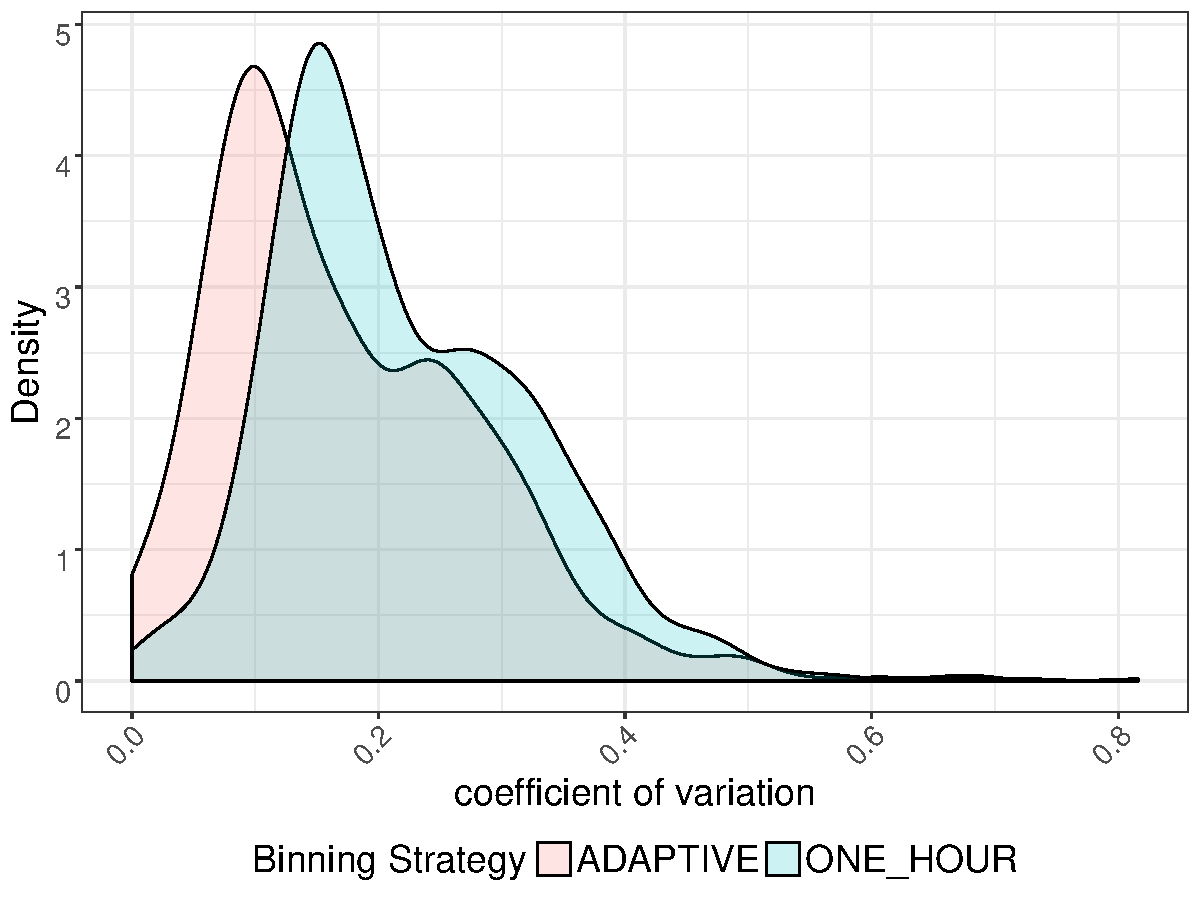
\includegraphics[width=\columnwidth,center,height=6cm,keepaspectratio]{images/COV.pdf}
	
	\caption{Adaptive vs fixed time buckets: Comparing the \ac{CoV} of adaptive and one hour time buckets during morning and evening peak hours for City~$1$.}
	\label{fig:compare-binning}
\end{figure}

In Figure~\ref{fig:compare-binning} we show the probability densities of \ac{CoV}\footnote{Coefficient of Variation defines the variation as a proportion of the mean and is given by $\frac{\sigma}{\mu}$, where $\mu$ and $\sigma$ are the sample mean and standard deviation.} for $20$ major roads in City~$1$ during the morning and evening peak hours. We can clearly see that using adaptive speed buckets helps to reduce the variance and hence obtain a more reliable (tighter) road speed profile estimate.


\subsection{Analysis of road speed distribution}
In this section, we present our analysis of road speeds over time intervals corresponding to peak and non-peak hours accumulated using our adaptive time buckets.

\label{subsec:speed-disribution}
\begin{figure}[!tb]
	\centering
	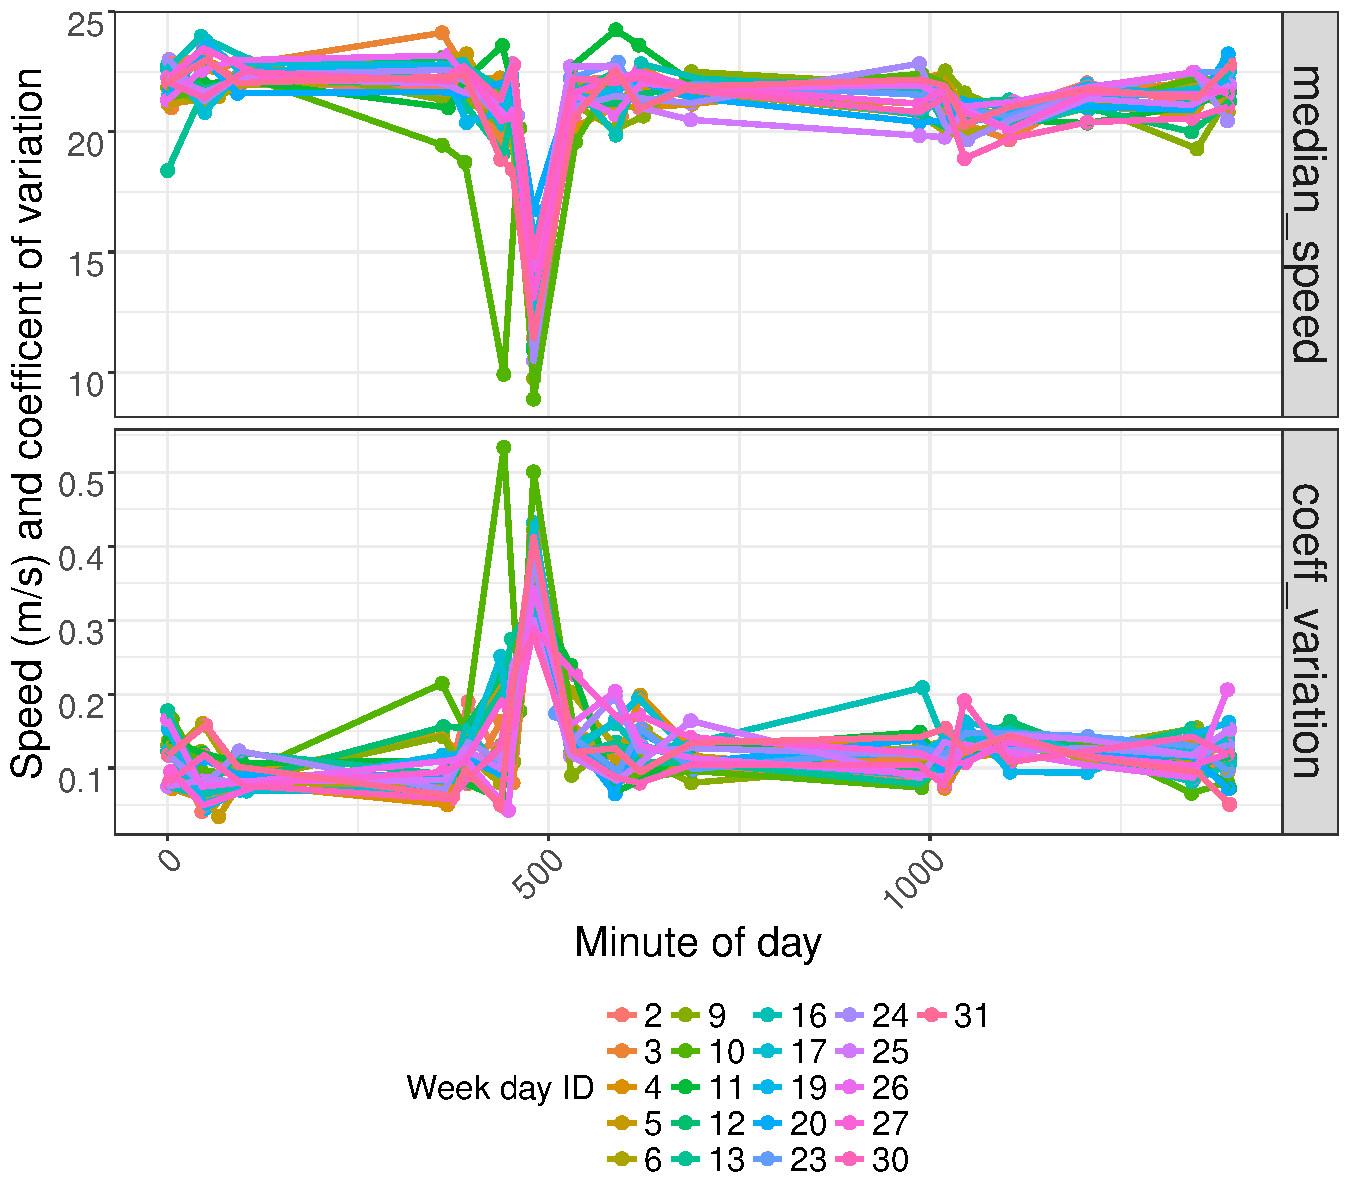
\includegraphics[width=\columnwidth,left]{images/AyerRajah.pdf}
	
	\caption{Variance in road speeds for an expressway in City~$1$}
	\label{fig:ayerajah-distribution}
\end{figure}

Figure~\ref{fig:ayerajah-distribution} shows the median speeds and the \ac{CoV}  for a few weekdays corresponding to the adaptive time bins for a $1.4$ km long road segment on an expressway in City~$1$. Figure~\ref{fig:ayerajah-distribution} clearly shows that the variance in traffic flow is much lower during non-peak hours compared to peak hours. The higher variance during peak hours can also be attributed to vehicles travelling in different lanes. For instance, vehicles exiting a congested off ramp from an expressway will slow down while vehicles on the remaining parallel lanes continue to move as usual.

\begin{figure}[!tb]
	\centering
	\subfloat[]{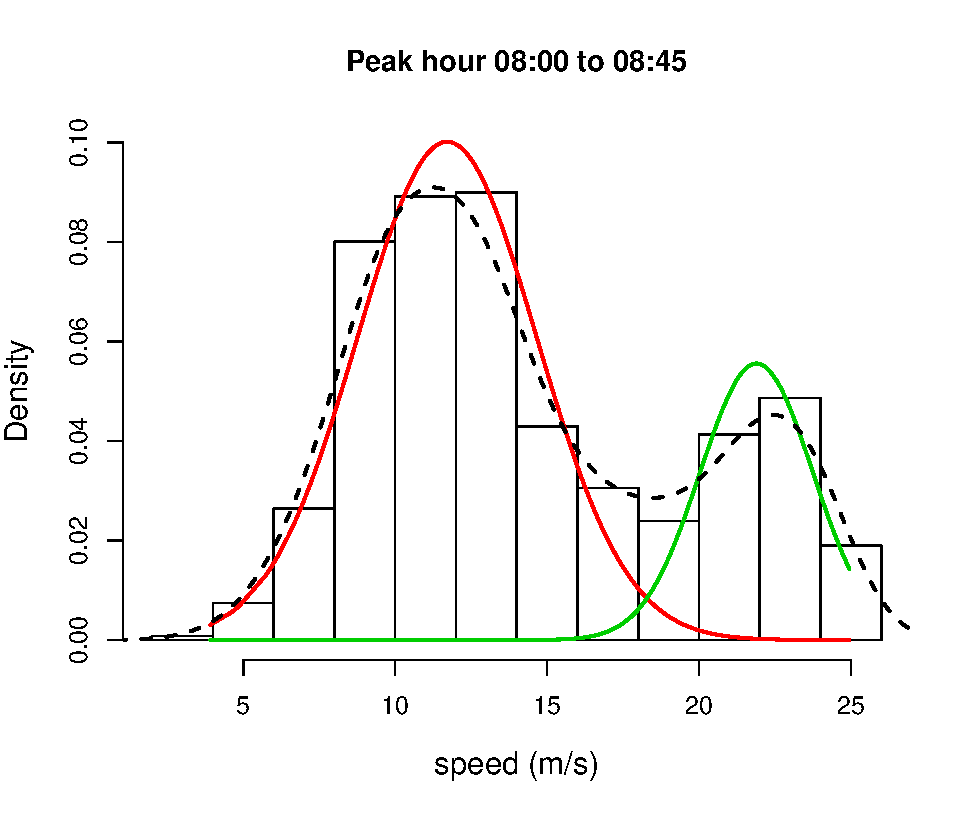
\includegraphics[width=.45\textwidth,center,height=5cm,keepaspectratio]{images/AYE-Peak.pdf}\label{fig:bimodal-peak}}
	\hfill%
	\subfloat[]{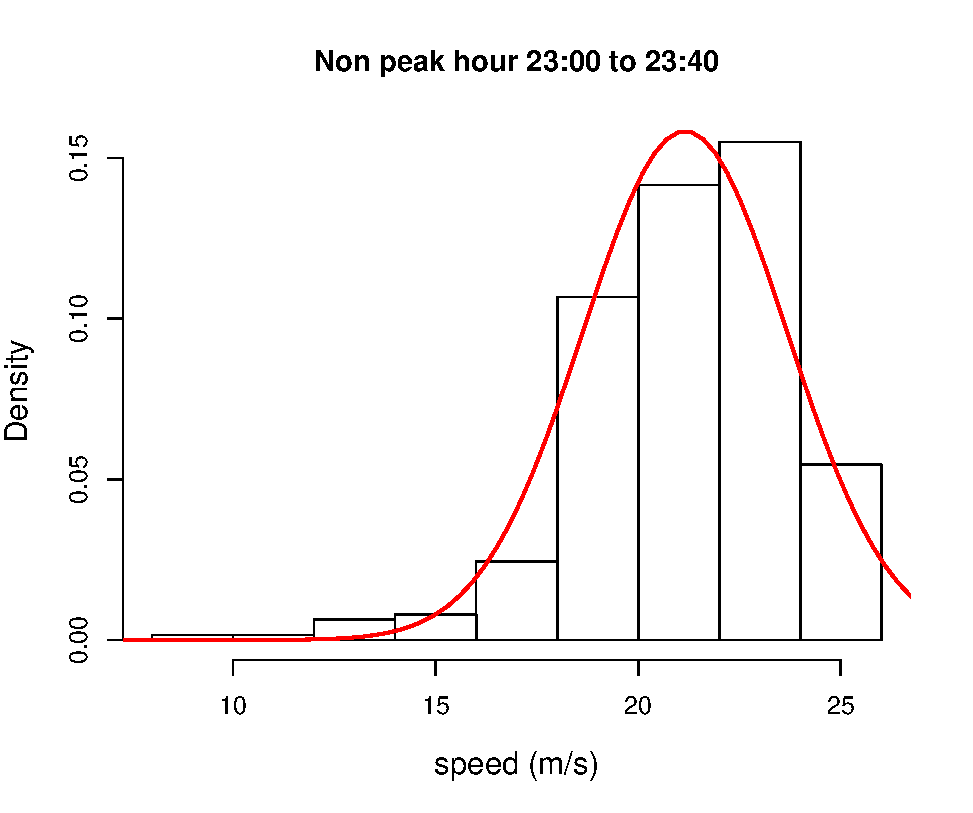
\includegraphics[width=.45\textwidth,center,height=5cm,keepaspectratio]{images/AYE-NonPeak.pdf}\label{fig:unimodal-nonpeak}}%
	\label{fig:speed-distributions}
	\caption{Speed distribution analysis: Distribution of vehicle speeds during (a) peak hours and (b) non peak hours for an expressway, clearly showing that peak-hour traffic exhibit high variance requiring a bi-modal distribution to model.}
\end{figure} 

In Figures~\ref{fig:bimodal-peak} and~\ref{fig:unimodal-nonpeak} we show the probability densities of speeds for the same expressway segment used in Figure~\ref{fig:ayerajah-distribution} during the morning peak and a random non-peak time intervals. We can clearly see that the distribution of vehicles speeds during the peak hours is bi-modal accounting for the large \ac{CoV}. The distribution of vehicle speeds during the non-peak time interval is as expected a Gaussian with very low variance. The implication of the analysis of road speed distribution is that it is much harder to predict travel times during peak hours largely due to the fact that vehicles in different lanes travel at different speeds depending upon the route.



Given this analysis on the vehicle speeds, we propose to compute the speed ranges for a road segment $e_i$ given by $\mu^{upper}_{e_i,t}$ and  $\mu^{lower}_{e_i,t}$ based on the Gosset's t-distribution with $68\%$ (two-tailed) confidence interval and $n-1$ degrees of freedom, when $\text{CoV}\le 0.3$. We assume that the vehicle speeds are IID (independent and identically distributed) normal. When the \ac{CoV} exceeds $0.3$ we assume that the distribution of the vehicle speeds is bimodal and use a Gaussian mixture model with two means   $\mu_{e_i,t}^{\text{d1}}$ and $\mu_{e_i,t}^{\text{d2}}$ which are used as proxies for the upper an lower bound speeds for the edge $e_i$ at time interval $t$. Note that the speed ranges are calculated for a road segment if there are at least a minimum $20$ driver location pings for a time interval. 



\subsection{Incremental learning using exponential moving averages}
\label{subsec:ema}
As in any production system, we need to update our speed profile models based on new data. In order to make our model update incrementally and in an online fashion, we use an exponential moving average to compute and update the speed ranges per road segment. Note that the \ac{RSP} per time interval (per day type) is computed every day.
From Figure~\ref{fig:ayerajah-distribution}, we can see that the median (along with mean and variance) speeds follow a recurring pattern on all weekdays. Although we observe a repetitive pattern on weekdays and weekends, it is important to keep the model updated as more are more cabs are added to our fleet and adapt to new changes such as addition of new roads and metro lines that change traffic conditions on the ground.
%
The \ac{EMA} based speed profiles helps us to continuously refine our \ac{RSP} estimates and  smooth out occurrences of anomalous speed values that could occur from time to time due to accidents, thunderstorms etc.



The \ac{EMA} for \ac{RSP} consisting of mean, median, upper and lower bound speeds per time interval per day of week is calculated using the Equation~\ref{eqn:ema} where $K=\frac{2}{N+1} \text{and } N \text{ is the length of the EMA}$.
\begin{equation}
\label{eqn:ema}
    \text{EMA}_\text{today}=\text{speed}_{\text{today}}\times K+\text{EMA}_\text{yesterday}\times(1-K)
\end{equation}

The length of \ac{EMA} window $N$ used for this study is $5$. The look-up table thus comprising \ac{EMA} of the \ac{RSP} is refreshed on a monthly basis.



\section{Travel time estimation}
\label{sec:travel-time-estimation}

\begin{figure}[!tb]
	\centering
	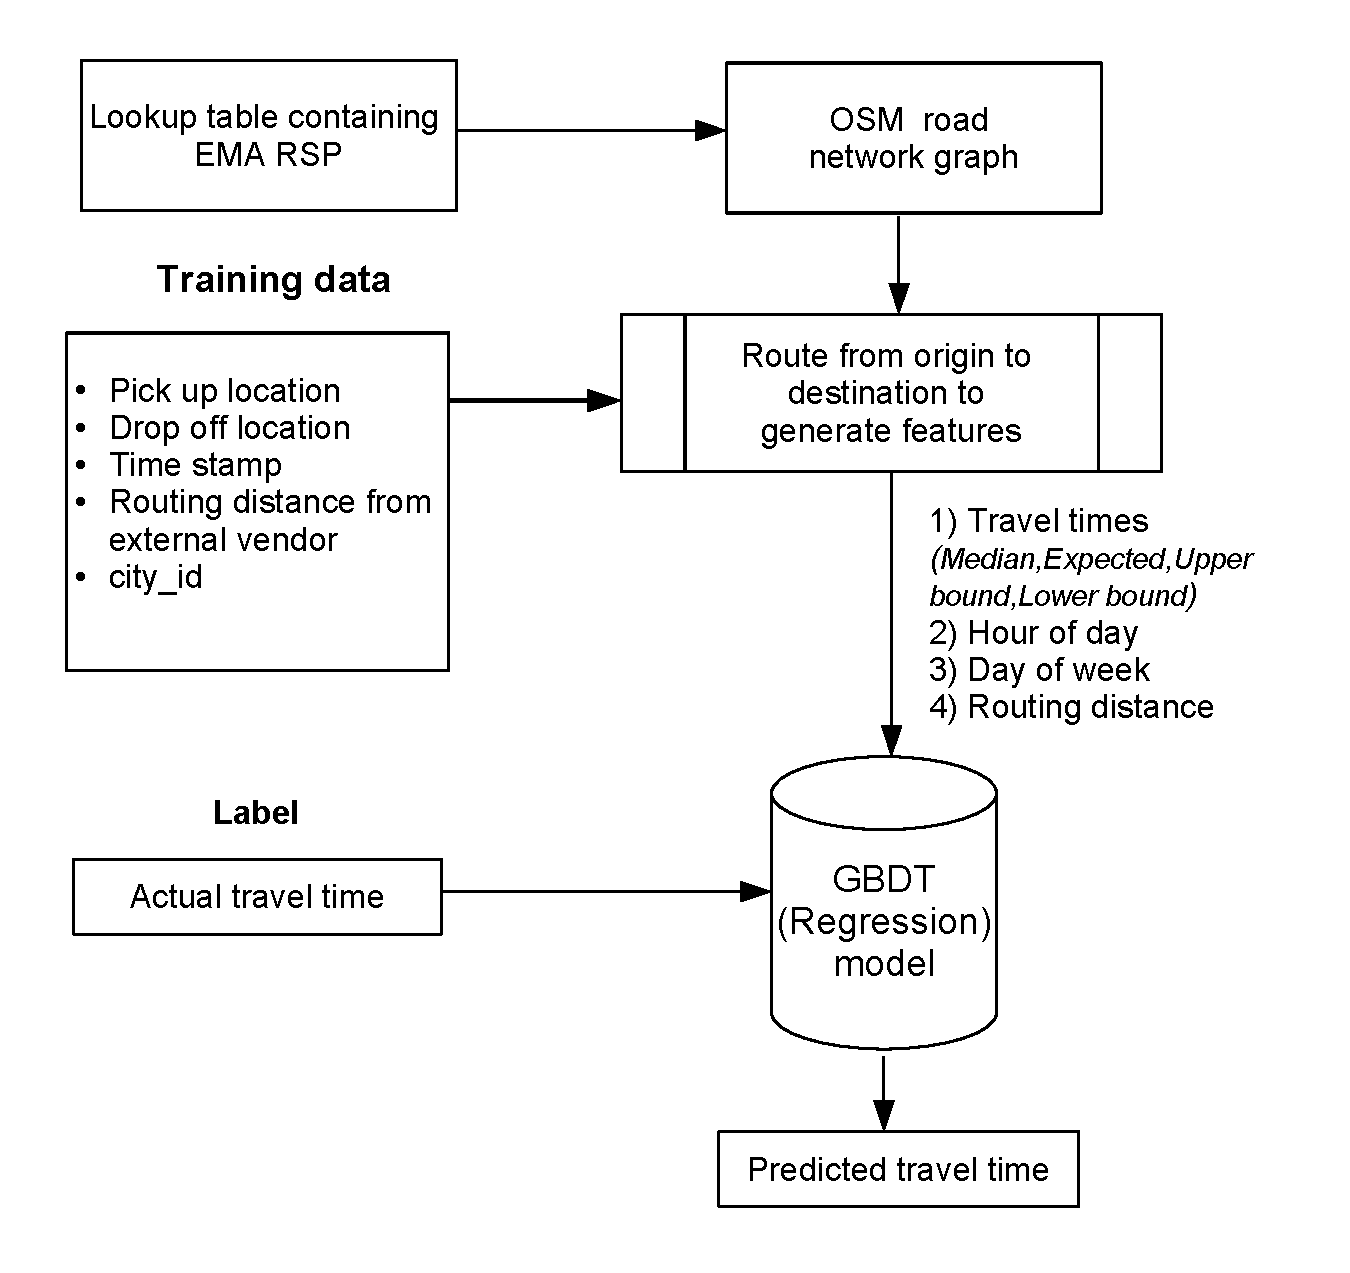
\includegraphics[width=\columnwidth,,height=7.5cm,center,keepaspectratio]{images/XgBoostCorrectiveModel.pdf}
	
	\caption{Gradient boosted decision trees (GBDT) model for correcting initial TTE estimate from road speed profiles.}
	\label{fig:xgboost-model}
\end{figure}

In this section we discuss how we leverage upon the \ac{RSP} and the corrective {\it GBDT}~\cite{schapire2003boosting} based regression model to compute the travel times. Given an \ac{OD} pair at a given time of the day and day of a week (weekday or weekend), we use the look-up table (created in the previous steps) to modify the weights of the road-network graph based on expected travel times across each edge of the \ac{OSM} road network graph. On computing the path between the ~\ac{OD} pair we get the expected, median, upper and lower bound travel times for the path from the look-up table. The values returned for \ac{TTE} from \ac{RSP} are the sum of the travel times across the edges constituting the path from the origin to destination.

The travel time estimates returned from the speed profiles are reasonably accurate during the non-peak hours and not very accurate during the peak hours. We have discussed reasons for this earlier in Section~\ref{subsec:speed-disribution}. 

The features that we use as inputs to the GBDT model to predict the final travel time \ac{OD} are  expected, median, lower bound and upper travel times (from \ac{RSP} look-up table and routing), day of the week and hour of the day. Note that separate GBDT models are trained for pickup and drop off phases per city. Figure~\ref{fig:xgboost-model} shows the work-flow for predicting the final travel time estimate given the output of \ac{RSP} as features to the corrective \ac{ML} model. 





\section{Experiments}
\label{sec:experiments}

\begin{table*}[!h]
\caption{Experimental results for two cities: Travel time estimates from road speed profiling and corrective \ac{ML} algorithm for City 1 and City 2 compared using MAPE, RMSE and BIAS.}
\centering
\begin{tabular}{|c|c|c|c|c|c|c|c|}
\hline
\multirow{3}{*}{\textbf{City}} & \multirow{3}{*}{\textbf{Phase}} & \multicolumn{6}{c|}{\textbf{Metric}}                                                                                                                                                                                                                                                                                                                                                                                                                                                          \\ \cline{3-8} 
                               &                                 & \multicolumn{2}{c|}{\textbf{MAPE}}                                                                                                                            & \multicolumn{2}{c|}{\textbf{RMSE}}                                                                                                                            & \multicolumn{2}{c|}{\textbf{Bias}}                                                                                                                            \\ \cline{3-8} 
                               &                                 & \textbf{\begin{tabular}[c]{@{}c@{}}Speed profiles\\ only\end{tabular}} & \textbf{\begin{tabular}[c]{@{}c@{}}After \\ corrective ML \\ algorithm\end{tabular}} & \textbf{\begin{tabular}[c]{@{}c@{}}Speed profiles\\ only\end{tabular}} & \textbf{\begin{tabular}[c]{@{}c@{}}After \\ corrective ML \\ algorithm\end{tabular}} & \textbf{\begin{tabular}[c]{@{}c@{}}Speed profiles \\ only\end{tabular}} & \textbf{\begin{tabular}[c]{@{}c@{}}After \\ corrective ML\\ algorithm\end{tabular}} \\ \hline
\multirow{2}{*}{City $1$}            & Pick up                         & 0.52                                                                   & 0.42                                                                                 & 122.84                                                                 & 100.66                                                                               & 29.97                                                                   & 22.11                                                                               \\ \cline{2-8} 
                               & Drop off                        & 0.21                                                                   & 0.145                                                                                & 261.19                                                                 & 172.61                                                                               & 175.13                                                                  & -6.745                                                                              \\ \hline
\multirow{2}{*}{City $2$}           & Pick up                         & 0.55                                                                   & 0.47                                                                                 & 193.27                                                                 & 162.84                                                                               & 40.05                                                                   & 33.03                                                                               \\ \cline{2-8} 
                               & Drop off                        & 0.27                                                                   & 0.18                                                                                 & 536.17                                                                 & 344.88                                                                               & 349.02                                                                  & 52.11                                                                               \\ \hline
\end{tabular}
\label{table:results}
\end{table*}



In this section, we evaluate the efficacy of road speed profiling, and assess the impact of the corrective Gradient Boosted decision tree~\cite{} algorithm on TTE. We evaluate this for both the phases of a trip commonly known in ride-hailing namely, i) the pickup phase, which is the time taken for the to reach the passenger for pickup after accepting the ride, and ii) drop off phase, which is the duration between passenger pickup and drop-off. Since these two phases have very different distributions, we train two separate ML models for correcting \ac{RSP} based travel time estimates. 

\textbf{Dataset:}
For generating the \ac{RSP} we used driver trajectories from close to $9.5$ million rides in (each)  City~$1$ and City~$2$ spanning 4 weeks. To train the corrective GBDT model for the pick up phase, we used $800$k train and $200$k test samples while  $1.3$ million train and $400$k test samples were used to train the model for the drop off phase.

\textbf{Features:}
The features to train the GBDT models are expected, median, upper and lower bound travel times and the routing distance (for an \ac{OD} pair) along with the minute of the day and day of the week of the trip. The label for the \ac{ML} model is the actual travel time from the origin to destination.

 

The metrics we use to evaluate the performance of the travel time estimates from \ac{RSP} and GBDT models against the actual travel times are as follows: 
\begin{enumerate}
\item \ac{MAPE} given by $\frac{1}{N}\sum_{i=1}^{N} \frac{abs(y_i-y_p)}{y_i}$

\item \ac{RMSE} given by $\sqrt{\frac{1}{N}\sum_{i=1}^{N} (y_i-y_p)^2}$

\item Bias given by $\frac{1}{N}\sum_{i=1}^{N} (y_i-y_p)$
\end{enumerate}
Where $y_i$ and $y_p$ represent the actual and predicted travel times for an \ac{OD} pair.

\subsection{Evaluation}
\label{subsec:results}
In this section we evaluate the performance of \ac{TTE} using the values from just road speed profiling and then followed by the corrective \ac{ML} model.

In Table~\ref{table:results} we summarize the results of road speed profiling and the corrective \ac{ML} models for City~$1$ and City~$2$ for the two phases of a cab ride. 

The results clearly show that the performance of both road speed profiling and corrective \ac{ML} model is superior in terms of \ac{MAPE} for the drop off phase compared to the pickup phase this is attributed to the greater uncertainty in the expected route a driver will take to pickup a passenger. We can also ascertain that the corrective \ac{ML} algorithm has significantly improved all the metrics compared to the output from \ac{RSP}. Finally the results of \ac{TTE} for City~$1$ is better than City~$2$ for all metrics considered. This can be attributed to City~$1$ having better infrastructure and lesser vehicle density resulting is less congestion.


\begin{figure}[!tb]
	\centering
	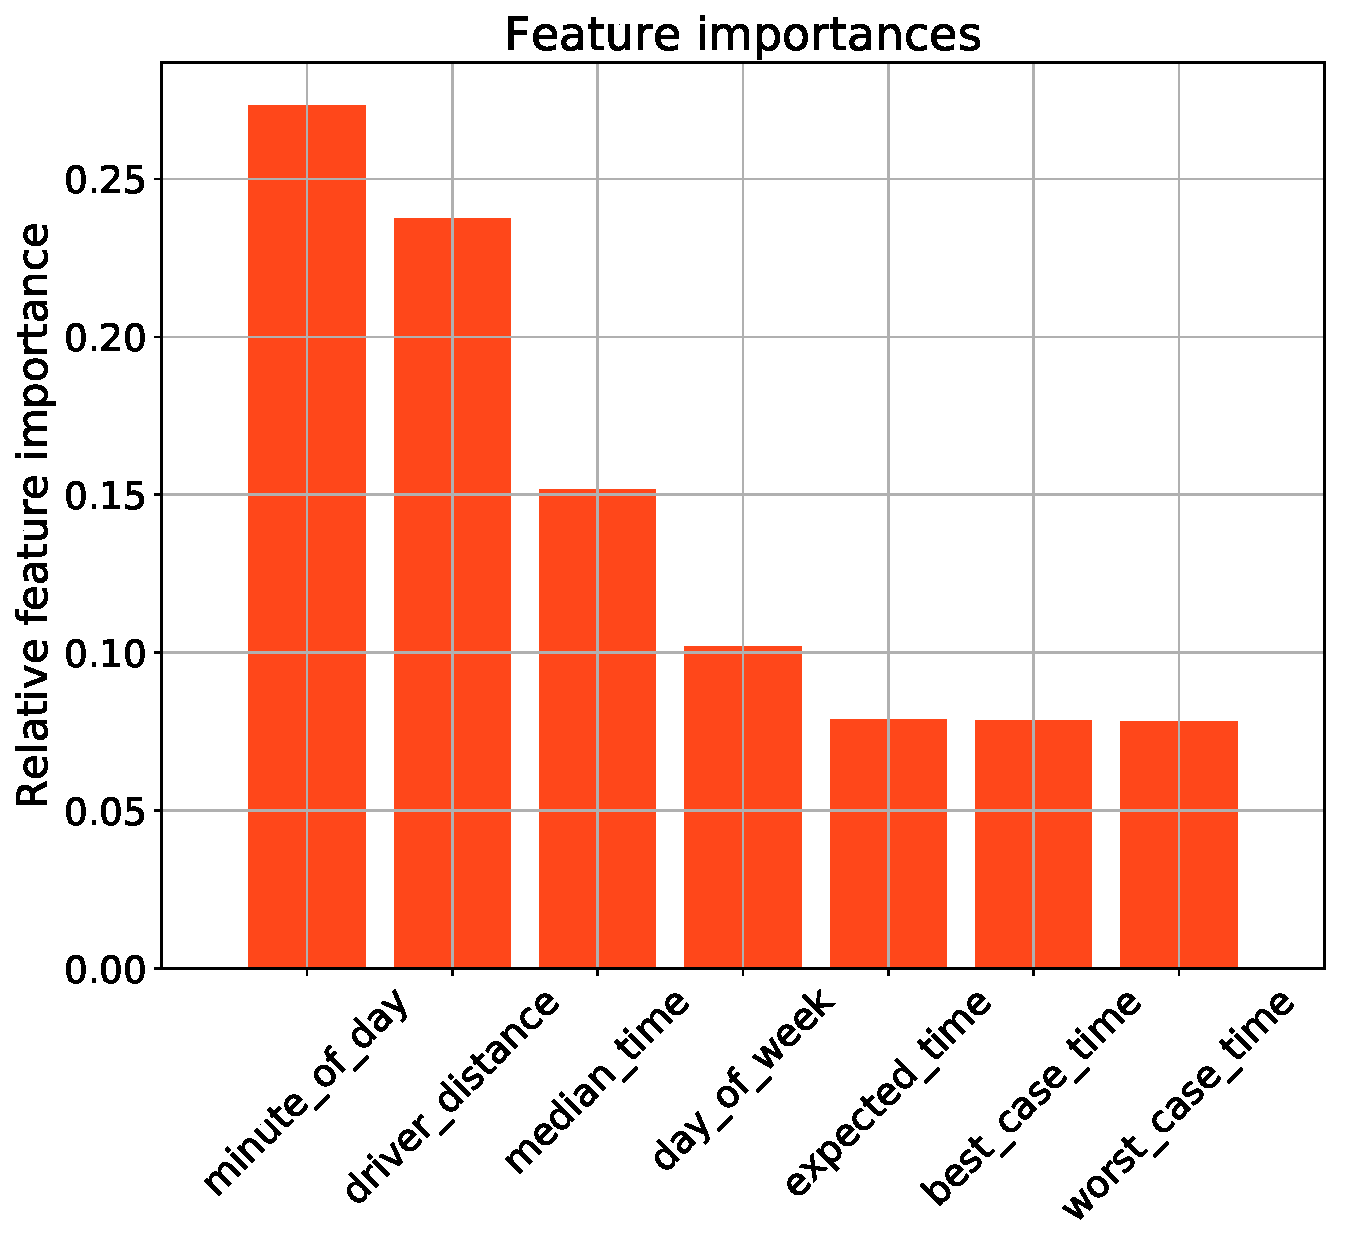
\includegraphics[width=\columnwidth,left,height=6.5cm,keepaspectratio]{images/feauture_importance.pdf}
	
	\caption{Relative feature importance from the GBDT model.}
	\label{fig:xgb-feature-importance}
\end{figure}



Figure~\ref{fig:xgb-feature-importance} shows the feature importance for one of the corrective GBDT models. Note that the order of feature importance in every GBDT model is the same. We see that the features \textbf{minute of the day} and the \textbf{driver distance} are the most important for correcting the \ac{RSP} travel time estimates. The former is important since the \ac{CoV} in speed profiles is dependent upon peak and non peak hours of the day. The driver distance is also an important feature for the corrective \ac{ML} model since we have seen that greater the distance between the \ac{OD} pairs more certain we are about the path that driver will take, thus resulting in better \ac{RSP} travel time estimates. Finally, we also observed that \textbf{median time} obtained from RSPs is also considered among the top-3 important features, proving the contribution of our inferred RSPs.  


\begin{figure}[!tb]
	\centering
	\subfloat[\ac{MAPE} over time of the day]{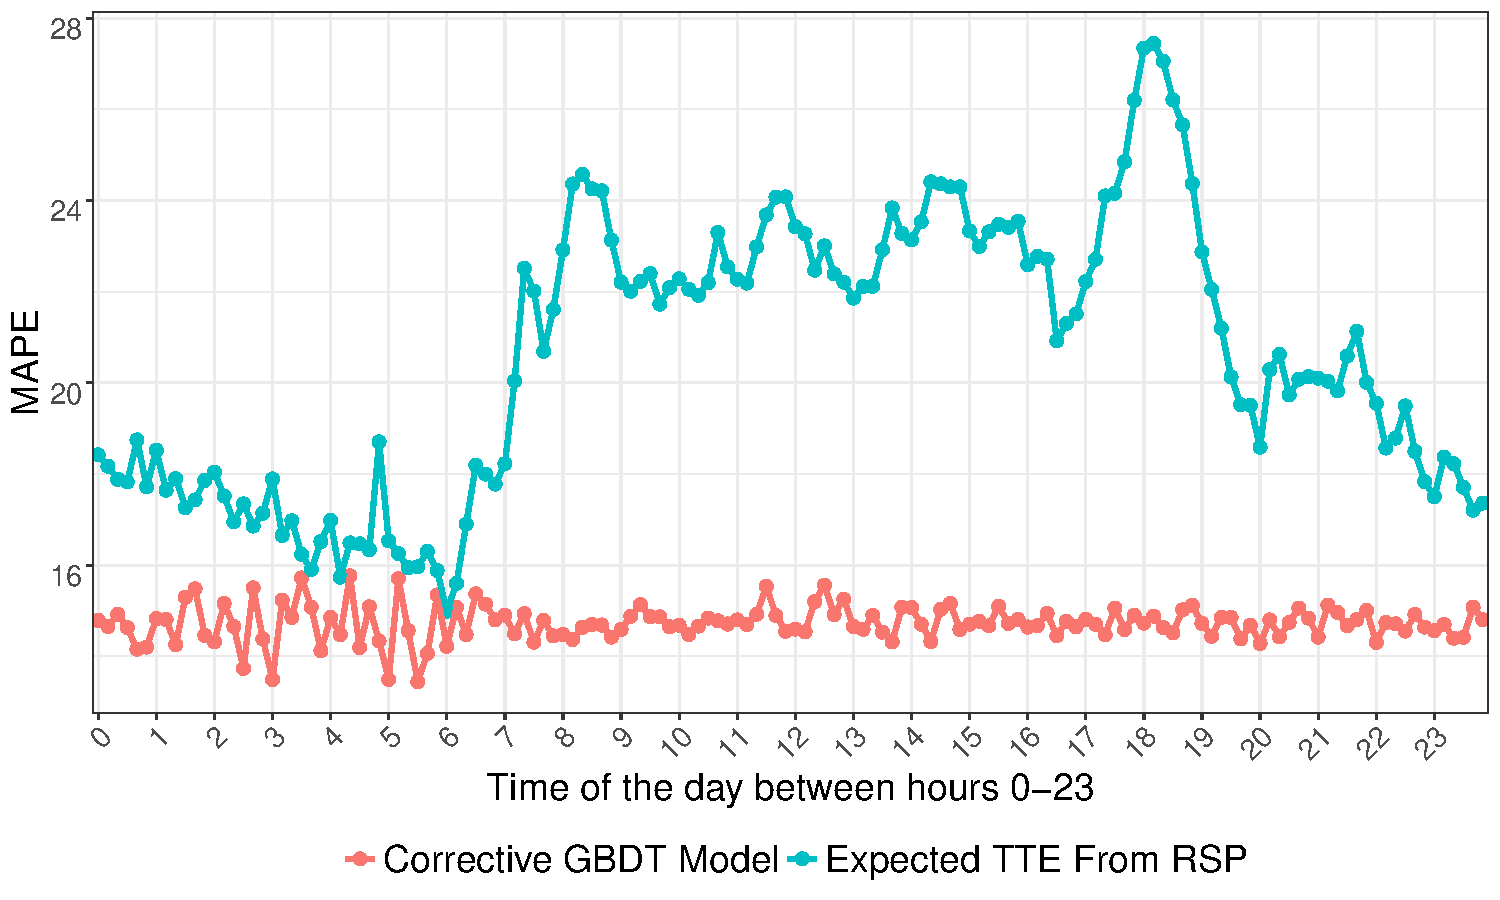
\includegraphics[width=\columnwidth,height=5.6cm,keepaspectratio]{images/ETT-TOD-SG.pdf}\label{fig:compare-rsp-xgboost-tod}}%
	\vfill%
	\subfloat[\ac{MAPE} over buckets (in km).]{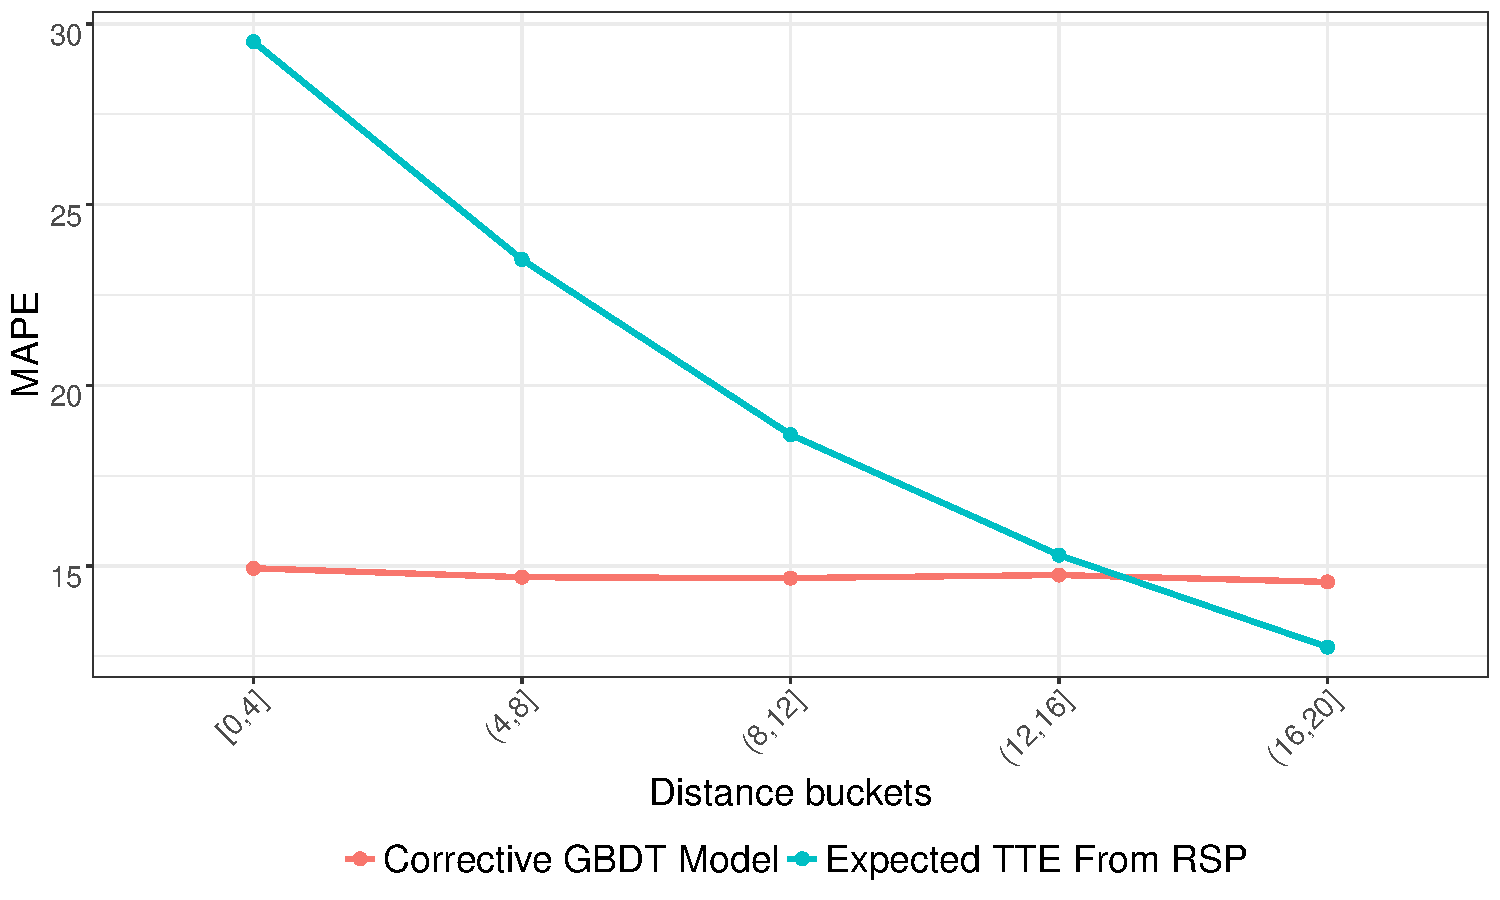
\includegraphics[width=\columnwidth,height=5.6cm,keepaspectratio]{images/ETT-Distance-SG.pdf}\label{fig:compare-rsp-xgboost-distance}}%
	\label{fig:eval-dropoff-sg}
	\caption{\ac{RSP} vs corrective GBDT model for the drop off phase in City $1$}
\end{figure} 

Figure~\ref{fig:compare-rsp-xgboost-tod} compares the performance of the expected travel time from \ac{RSP}  with that of the corrective GBDT model which takes the output of \ac{RSP} as input for City $1$ over an entire day. We can see that travel time estimates from \ac{RSP} have varying accuracy based on time of day. MAPE for estimates during non peak hours is less compared to that of peak hours, which could be attributed to large variance in traffic flow (as discussed in Section~\ref{subsec:speed-disribution}) that is not captured by RSPs, perhaps with the given data. The performance of  GBDT model tends to have less variance over time, indicating that GBDT captures non-linearities in traffic flow and time dependencies well in order to correct the errors in \ac{RSP}. 


Figure~\ref{fig:compare-rsp-xgboost-distance} compares the performance of \ac{RSP} with GBDT model for different distance buckets during the drop off phase for City $1$. We can see that the performance of the expected speed from \ac{RSP} becomes better as the distance of the ride increases. This can be attributed to the fact that we tend to predict the path for an \ac{OD} pairs that are far apart with better accuracy than for OD pairs that are close by. Note that knowing the exact path taken by the driver plays a crucial role in using RSP for TTE. For shorter rides there are multiple paths that can be taken from the origin to destination. This is amplified further by inaccuracies in \ac{OSM}'s routing especially seen for shorter rides. Performance of the GBDT model is again distance invariant. We notice that the performance of the GBDT gets worse than the RSP based estimates for  $16-20$ km distance bucket since we have very few rides in that bucket in our training data. 
This indeed highlights the limitations and merits of GBDT based approach and RSP based approach respectively.  

\begin{figure}[!tb]
	\centering
	\subfloat[\ac{MAPE} over time of the day]{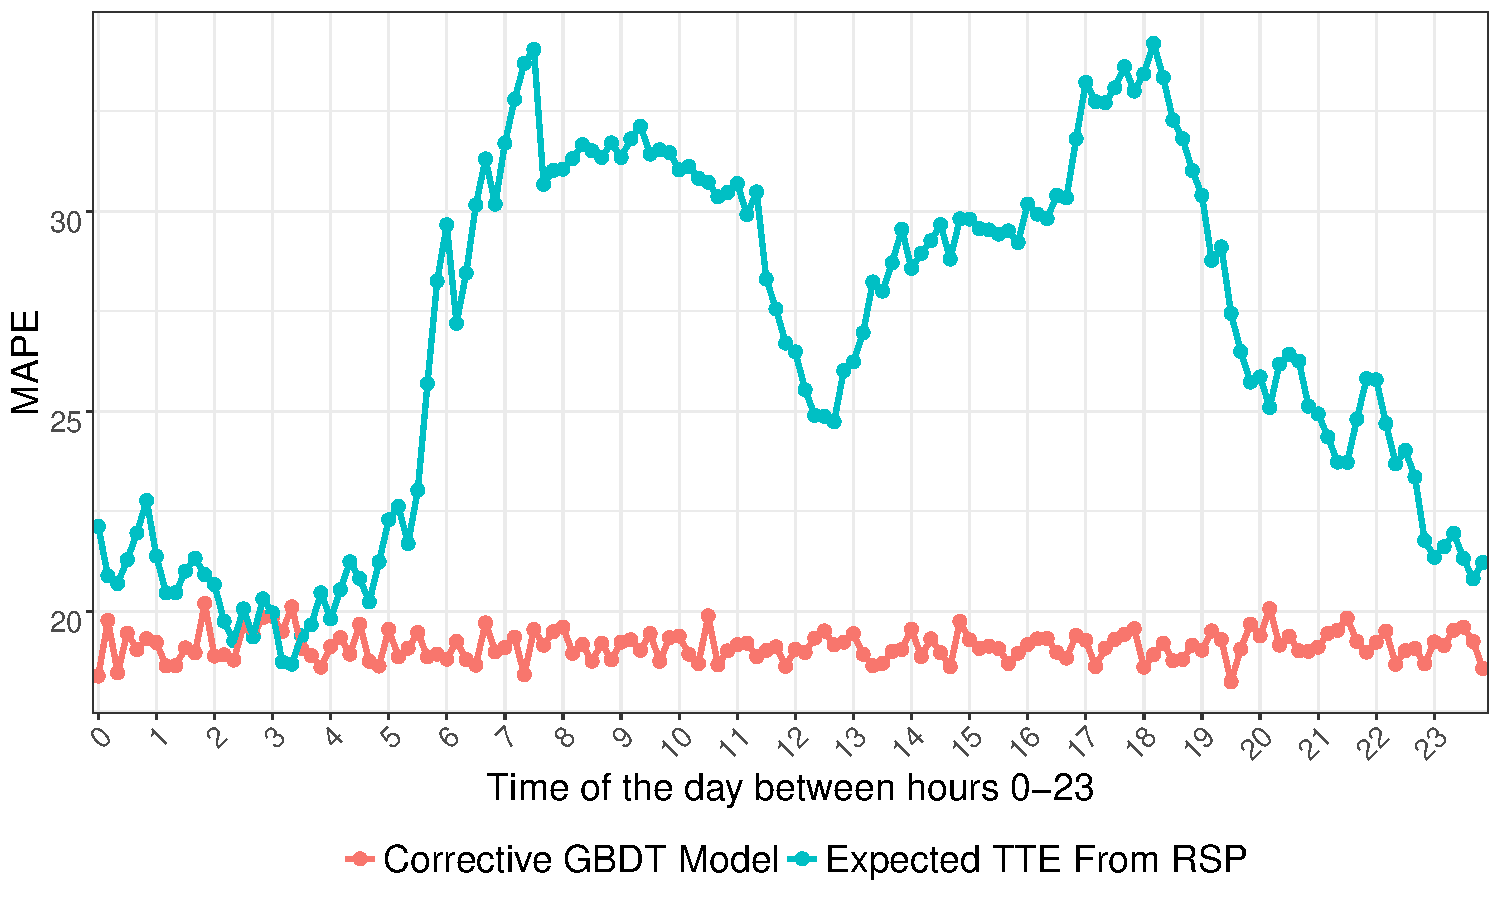
\includegraphics[width=\columnwidth,height=5.6cm,keepaspectratio]{images/ETT-TOD-MNL.pdf}\label{fig:compare-rsp-xgboost-tod-mnl}}%
	\vfill%
	\subfloat[\ac{MAPE} over buckets (in km).]{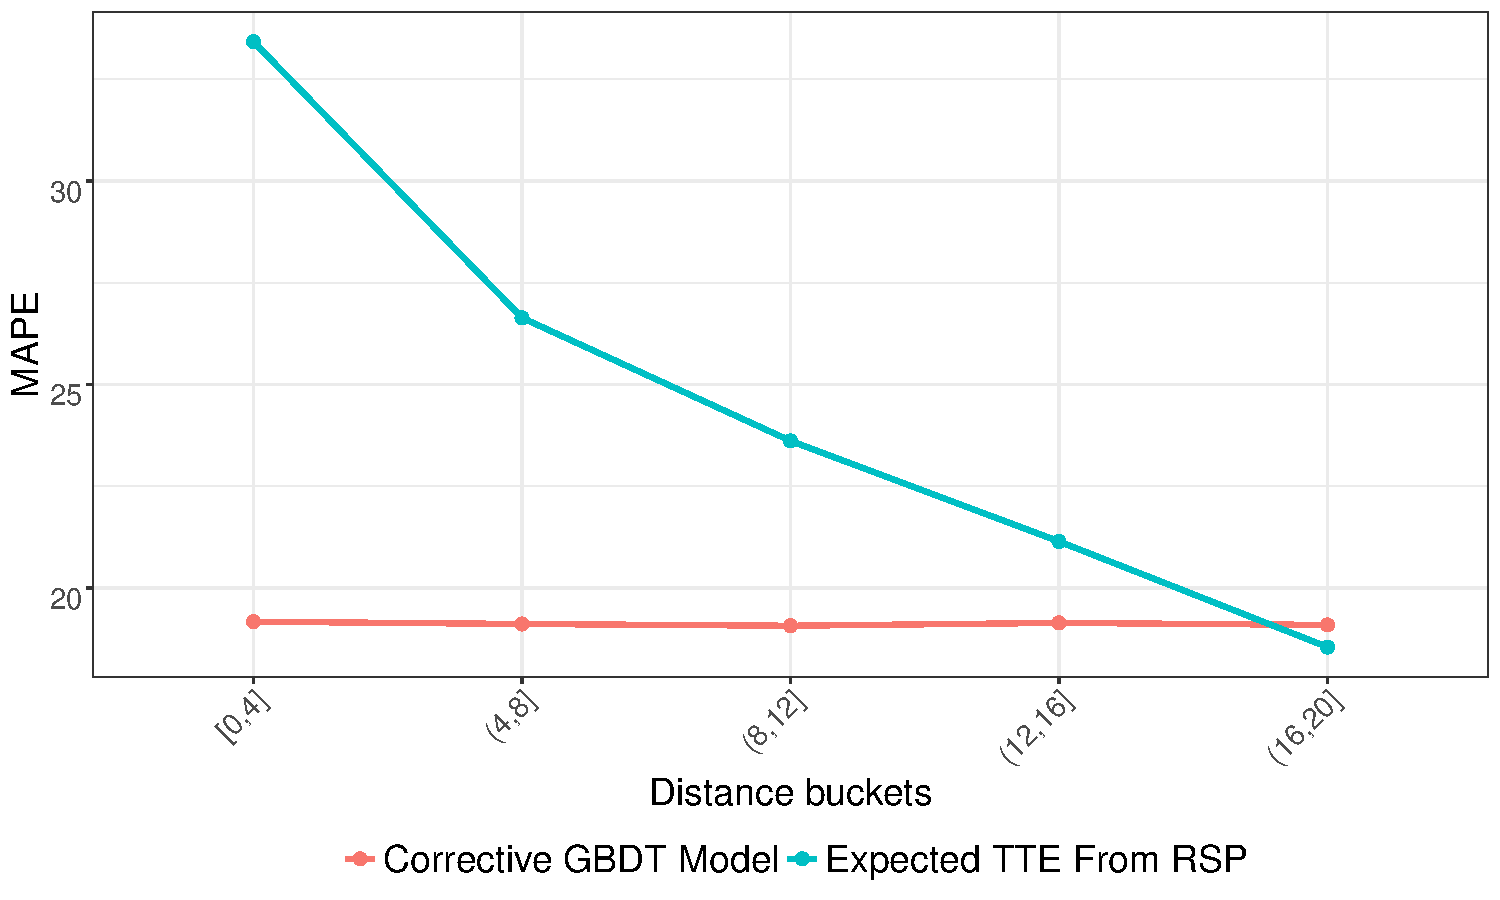
\includegraphics[width=\columnwidth,height=5.6cm,keepaspectratio]{images/ETT-Distance-MNL.pdf}\label{fig:compare-rsp-xgboost-distance-mnl}}%
	\label{fig:eval-dropoff-mnl}
	\caption{\ac{RSP} vs corrective GBDT model for the drop off phase in City $2$}
\end{figure} 

A similar comparison, i.e., performance of the expected travel time from \ac{RSP} vs GBDT based corrective model for the drop off phase in City $2$, 
is presented in figures~\ref{fig:compare-rsp-xgboost-tod-mnl} and~\ref{fig:compare-rsp-xgboost-distance-mnl}. The conclusions that we can derive from the plots for City $2$ are the same for City $1$. As noted in Table~\ref{table:results} we can see that \ac{RSP} estimates and GBDT model performance are inferior for City $2$ compared to City $1$.


\section{Conclusions}
\label{sec:conclusion}

In this work, we presented a model for travel time estimation that relies on modeling \ac{RSP} for individual road segments. Our analysis of vehicle speed distribution across different times of the day showed that vehicle speeds tend to have large variance during peak-hours compared to non-peak hours. In order to arrive at RSP with tight confidence intervals, we proposed decision tree based dynamic time buckets to accumulate speed observations. An exponential moving average is then used to incrementally update RSPs with incoming observations. Finally, in order to provide an accurate TTE, we adopted a hybrid approach, where a gradient boosted decision tree learning algorithm is trained on inputs including initial TTE from RSPs, along with time and day. Experimental evaluation done on taxi trip data coming from historical trips in two large cities of S.E Asia show that our initial TTE is a valuable feature that can be further refined or bias-corrected by the ML model. We observe this improvement consistently across both pickup and drop off phases of ride-hailing. To the best of our knowledge, our work is one of the first works to study the problem of large scale traffic state estimation and \ac{TTE} in S.E Asia using big data. 

 











% Can use something like this to put references on a page
% by themselves when using endfloat and the captionsoff option.
\ifCLASSOPTIONcaptionsoff
  \newpage
\fi


%\begin{thebibliography}{1}
\bibliographystyle{IEEEtran}
\bibliography{ICDMAbhinav2018} 


\end{document}


